\documentclass[a4paper,12pt,numbers=enddot]{scrreprt}	% numbers=enddot fa seguire il puntino dopo il numero di cap. noenddot lo toglie 
\usepackage[utf8]{inputenc}	%imposta la codifica di input; invece di "latin1", anche "utf8" va bene
\usepackage[footnotesize,it]{caption}	%per i cara piccoli
\usepackage[english]{babel}	%l?ultima lingua � quella predefinita
\usepackage{listings}		%codice sorgente
\lstset{frame=shadowbox, rulesepcolor=\color{blue}, breaklines=true, basicstyle=\small\ttfamily, columns=fullflexible,  keepspaces=true}	%disegna un rettangolo attorno al codice sorgente
\usepackage{indentfirst}	%rientra il primo paragrafo di ogni sezione
\usepackage{amsmath}%,amssymb,amsthm       % indispensabili per la matematica
\usepackage{graphicx}		% per inserire le immagini
\usepackage{graphics}		%?
\usepackage{sidecap}		%per mettere caption a lato della figuta
 % didascalie personalizzate
\usepackage{caption}		
\usepackage[numbers]{natbib} %?
\usepackage{psfrag} %?
\usepackage{multirow}	%?
\usepackage{booktabs} 	%?
\usepackage{lscape}%?
\usepackage{longtable}%?  %%
\usepackage{enumitem}%?
\usepackage{epsfig}		%per mettere fig usando comando tabular
\usepackage{makeidx}	%indice
\usepackage{varioref}
\usepackage[table]{xcolor}
\usepackage{epstopdf}
\usepackage{wrapfig}
%Setta dimensioni body
\usepackage[total={16.5cm,25cm},
						top=3.5cm,
						bottom=3.5cm,
						left=2.5cm,
						right=2.5cm,
						%includefoot,
						centering]{geometry}

\usepackage{wallpaper}%?
\usepackage{color}%?
\usepackage{setspace}		%per definire con dopo l'interlinea con \onehalfspacing
\onehalfspacing
\usepackage{appendix}
\usepackage{acronym}%?
\usepackage{makecell}

%Intestazioni e pie? pag.  
\usepackage[automark,headsepline,footsepline,autooneside,plainheadsepline,plainfootsepline]{scrpage2}	%i comandi plain-ecccc servono a dire che nella prima pag. del nuovo cap. voglio queste cose.
\usepackage[pagebackref=true, colorlinks=true, linkcolor=blue, hyperindex=true, urlcolor=blue, citecolor = green, linktocpage=true]{hyperref}		% indici e riferimenti cliccabili
\pagestyle{scrheadings}
\clearscrheadfoot
\ihead [Francesco Bonfadelli]{Francesco Bonfadelli}	%Kopfzeile Innen
\chead {}					%Kopfzeile Mitte
\ohead [\headmark]{\headmark}			%Kopfzeile Au�en
\ifoot {}					%Fu�zeile Innen
\cfoot[\pagemark]{\pagemark} 			%Fu�zeile Mitte
\ofoot {}

\automark[chapter]{chapter}
\KOMAoptions{cleardoublepage=scrheadings}	%per lasciate style=scrheadings anche per le pag vuoto (svuotate col comando cleardoublepage), si puo? anche scegliere cleardoublepage=plain o empty

\footskip=30pt	 %	abbassa il margine inf della pag
\setlength{\headheight}{2\baselineskip}

\newcommand\SectionFontStyle{\rmfamily}			% geh�rt zu den beiden folgenden setkomafont , keine ahnung was es macht =)
\setkomafont{chapter}{\huge\bfseries\SectionFontStyle}	% Chapter in der gleichen schriftart SectionFontStyle
\setkomafont{sectioning}{\bfseries\SectionFontStyle}
%Crea i link nel pdf (vedere come si fa a farli verdino e con i collegamenti solo sui numeri, non questi rettangoli cessi rossi	

\makeindex
\begin{document}

\renewcommand{\bibname}{References}	%to change the name: bibliography to references

%\pagenumbering{roman}
%\pagestyle{plain}
%******************************************************************
% Materiale iniziale
%******************************************************************

\begin{titlepage}   %Frontespizio
\begin{center}
{\Large UNIVERSIT\`A DEGLI STUDI DI BRESCIA}

\vspace{0.2cm}

{\Large FACOLT\`A DI INGEGNERIA}

\begin{figure*}[htbp] 
\begin{center}
 \begin{tabular}{c c}
\raisebox{-.5\height}{
\includegraphics[width=0.20\textwidth]{images/00-loghi/logo_UniBS.eps}}
 & \raisebox{-0.57\height}{
\includegraphics[width=0.20\textwidth]{images/00-loghi/freiburg.png}}
\end{tabular}
\end{center}
\end{figure*}

% \vspace{0.5cm}

CORSO DI LAUREA MAGISTRALE IN INGEGNERIA INFORMATICA \\

%TESI DI LAUREA SPECIALISTICA \\

%\vspace{0.8cm}
\vspace{1.5cm}
{\normalsize \emph{\textbf{ESTRAZIONE AUTOMATICA DI INFORMAZIONE}}} \\

\vspace{0.2cm}

{\normalsize \emph{\textbf{SIMBOLICA DA IMMAGINI}}} \\

%\vspace{0.2cm}

%{\normalsize \emph{\textbf{PER COMPITI DI NAVIGAZIONE}}} \\

%{\normalsize \emph{\textbf{IN REGIME INTERMITTENTE}}} \\

\vspace{0.5cm}

{\small \emph{\textbf{(Automatic extraction of symbolic information from images)}}} \\

\vspace{1.5cm}

\begin{flushleft}

{\normalsize Relatore:}
\begin{quote}
{\large \textbf{Ch.mo Prof. Riccardo Cassinis}} \\
\vspace{0.2cm}
\end{quote}

{\normalsize Correlatore:}
\begin{quote}
{\large \textbf{Ch.mo Prof. Marco Ragni}} \\
\vspace{0.2cm}
\end{quote}

\end{flushleft}

% \vspace{0.5cm}

\begin{flushright}
Laureando: \\
\textbf{Francesco Bonfadelli} \\
\vspace{0.05cm}
\textbf{Matricola 83174} \\
\vspace{1.5cm}
\end{flushright}

\large{Anno Accademico 2012-2013}

\end{center}
\end{titlepage}


\pagenumbering{arabic}
\tableofcontents
\listoffigures

\newpage
\thispagestyle{empty}
\mbox{}

\chapter{State Of The Art}
  This chapter, after having introduced the concept of cognitive architecture, describes the main working instrument used for this work: \mbox{ACT-R,} the cognitive architecture and \mbox{OpenCV,} the computer vision library. 
  %% Cognitive Architecture
  \section{Cognitive Architecture}	
	A cognitive architecture is the implementation through computer simulation softwares \todo{controllare correttezza di softwares} of a theory about human cognition. The theory generally relies on a wide selection of human experimental data. The design of these architectures tries to simulate human intelligence in a humanlike way.
	
	\textit{"A cognitive architecture is not a single algorithm or method for solving a problem; rather, it is the task-independent infrastructure that brings an agent’s knowledge to bear on a problem in order to produce behavior"}~\cite{SoarCogArch2012}. A cognitive architecture alone can not solve any problem. In order to be able to do it, it needs to be supplied with the knowledge to perform it. The combination of an architecture and the knowledge necessary to solve a specific task is called \emph{model}. It is possible to create many models able to solve the same task. The specific knowledge is determined by the \emph{modeler} ~\cite{Sears2012}. 
	
	Another important feature of cognitive architectures is that they give the possibility to make comparison between the sequence of actions produced by the model and the ones produced by human beings when they try to solve the same task. In addition, the measured quantities can be not only qualitative ones, like the correctness of the goal, but also quantitative, as for example, the time necessary to complete a task. This gives the models the possibility to produce execution times, error rates and learning curves. Comparisons with human performances can be useful to evaluate the quality of model ~\cite{Sears2012}. 
	
	As the term \emph{infrastructure} suggests, cognitive architectures usually are built aggregating many software modules, most of which represent functions of the human brain. Anyway, there exist other modules, which coordinate the overall functioning and without which the whole architecture could not work. In the following section, which describes \emph{ACT-R}, the \emph{procedural module} is an example of such modules. In fact, it does not represent a function of the human being, though it is necessary to coordinate the communication between all the other modules. 
	
	Some architectures, can, in addition, include some \emph{learning mechanisms}. This can be the attempt to simulate the human memory system, thanks to which the behaviour of a human can be different after having experienced facts or consequences of a specific choice ~\cite{Sears2012}.
	
	
  %% ACT-R
  \section{ACT-R}
	\mbox{ACT-R}, that stands for \emph{Adaptive Control of Thought-Rational}, is a cognitive architecture that implements the homonym theory developed by John Robert Anderson, professor of psychology and computer science at Carnegie Mellon University. 
	\mbox{ACT-R} is a software written in Lisp and its models are written in a Lisp-like language. It is thought to have a modular structure so that it can be easily extended. The current version of the software is the 6.0. \todo{mancano le fonti praticamente ovunque}
		
	\subsection*{Basic concept of ACT-R's theory}
	In psychology, memory is defined as the processes by which information is encoded, stored, and retrieved ~\cite{baddeley2009memory}. 
	
	\mbox{ACT-R's} most important assumption about knowledge is based on Anderson's theory about memory. 
	Anderson, divides memory into \emph{declarative} and \emph{procedural}. 
	Declarative memory refers to all the memories that can be consciously recalled. This kind of knowledge comprehends facts and knowledge that human beings explicitly know. To call back this kind of information, there must be a conscious process by the human being. For this reason, this kind of memory is also called \emph{explicit}.
	In contrast, procedural memory refers to all that notions or skills that human beings have but which they learnt in an implicit way. Examples of this knowledge are, for example, driving, reading and writing. In this case, in order to call back this kind of information, the human being does not need a conscious process. That is why this kind of memory is also called \emph{implicit} ~\cite{anderson1976language}. 
	
	The following example is used to explain better how these two kinds of memory work. 
	When a person starts learning typewriting, an attempt he can make in the beginning is trying to memorize the layout of the keyboard. The knowledge of all the positions of the keys is the declarative memory. After having become a skilled typewriter, the same person will write quickly putting his fingers in the right keys and pushing them in the correct order without thinking anymore about the positions of the keys on the keyboard. Moreover, if we ask him where the position of a certain character is on the keyboard, he will probably answer that he can not say it without looking at it. This is because, now, he is using his procedural memory ~\cite{anderson1993rules}.
	
	\subsection*{Architecture}
	In \mbox{ACT-R}, declarative memory is represented in structures, called \emph{chunks}, and procedural memory is represented as rules, called \emph{productions}. Chunks and productions are the basic building blocks of an ACT-R model ~\cite{actr6refman}.
	
	The \emph{chunks} are data structures which are defined by their \emph{type} and their \emph{attribute list}, that is a tuple of pairs, each of which is called \emph{slot} and is composed by the \emph{name} of the attribute, which is fixed for a certain chunk, and the \emph{value} of the attribute, which, instead, can assume different values. Each chunk has also a \emph{name} but it is not considered to be a part of the chunk itself, as it does not exist in \mbox{ACT-R} theory. It is used only for convenience to reference the specific chunk when writing models. The chunk-types can be organized into hierarchies ~\cite{actr6refman}.
	
	The \emph{productions} are the \mbox{ACT-R} equivalent of functions. They define sequences of actions and can be fired only if a set of preconditions is satisfied. They can be represented as \emph{if-then} rules, where the \emph{if-part} is a set of conditions that must be true for the production to apply and the \emph{then-part} is the action of the production and consists of the operations the model should perform when the production is selected and used ~\cite{actr6refman}.
	\newline{}

	
	All the activities carried out by the human brain, like talking or moving, are performed by neurons located close together, in a well defined and limited area of the cortex. Trying to imitate this "architecture", \mbox{ACT-R's} framework is structured in different \emph{modules}, each of which represents one specific function of the human brain. 
	
	
	
	In the \mbox{ACT-R's architecture} the task of the procedural module is to coordinate all the other modules. The exchange of information between the modules is achieved through \emph{buffers}.

	\begin{figure}[h]
	  \begin{center} 
	    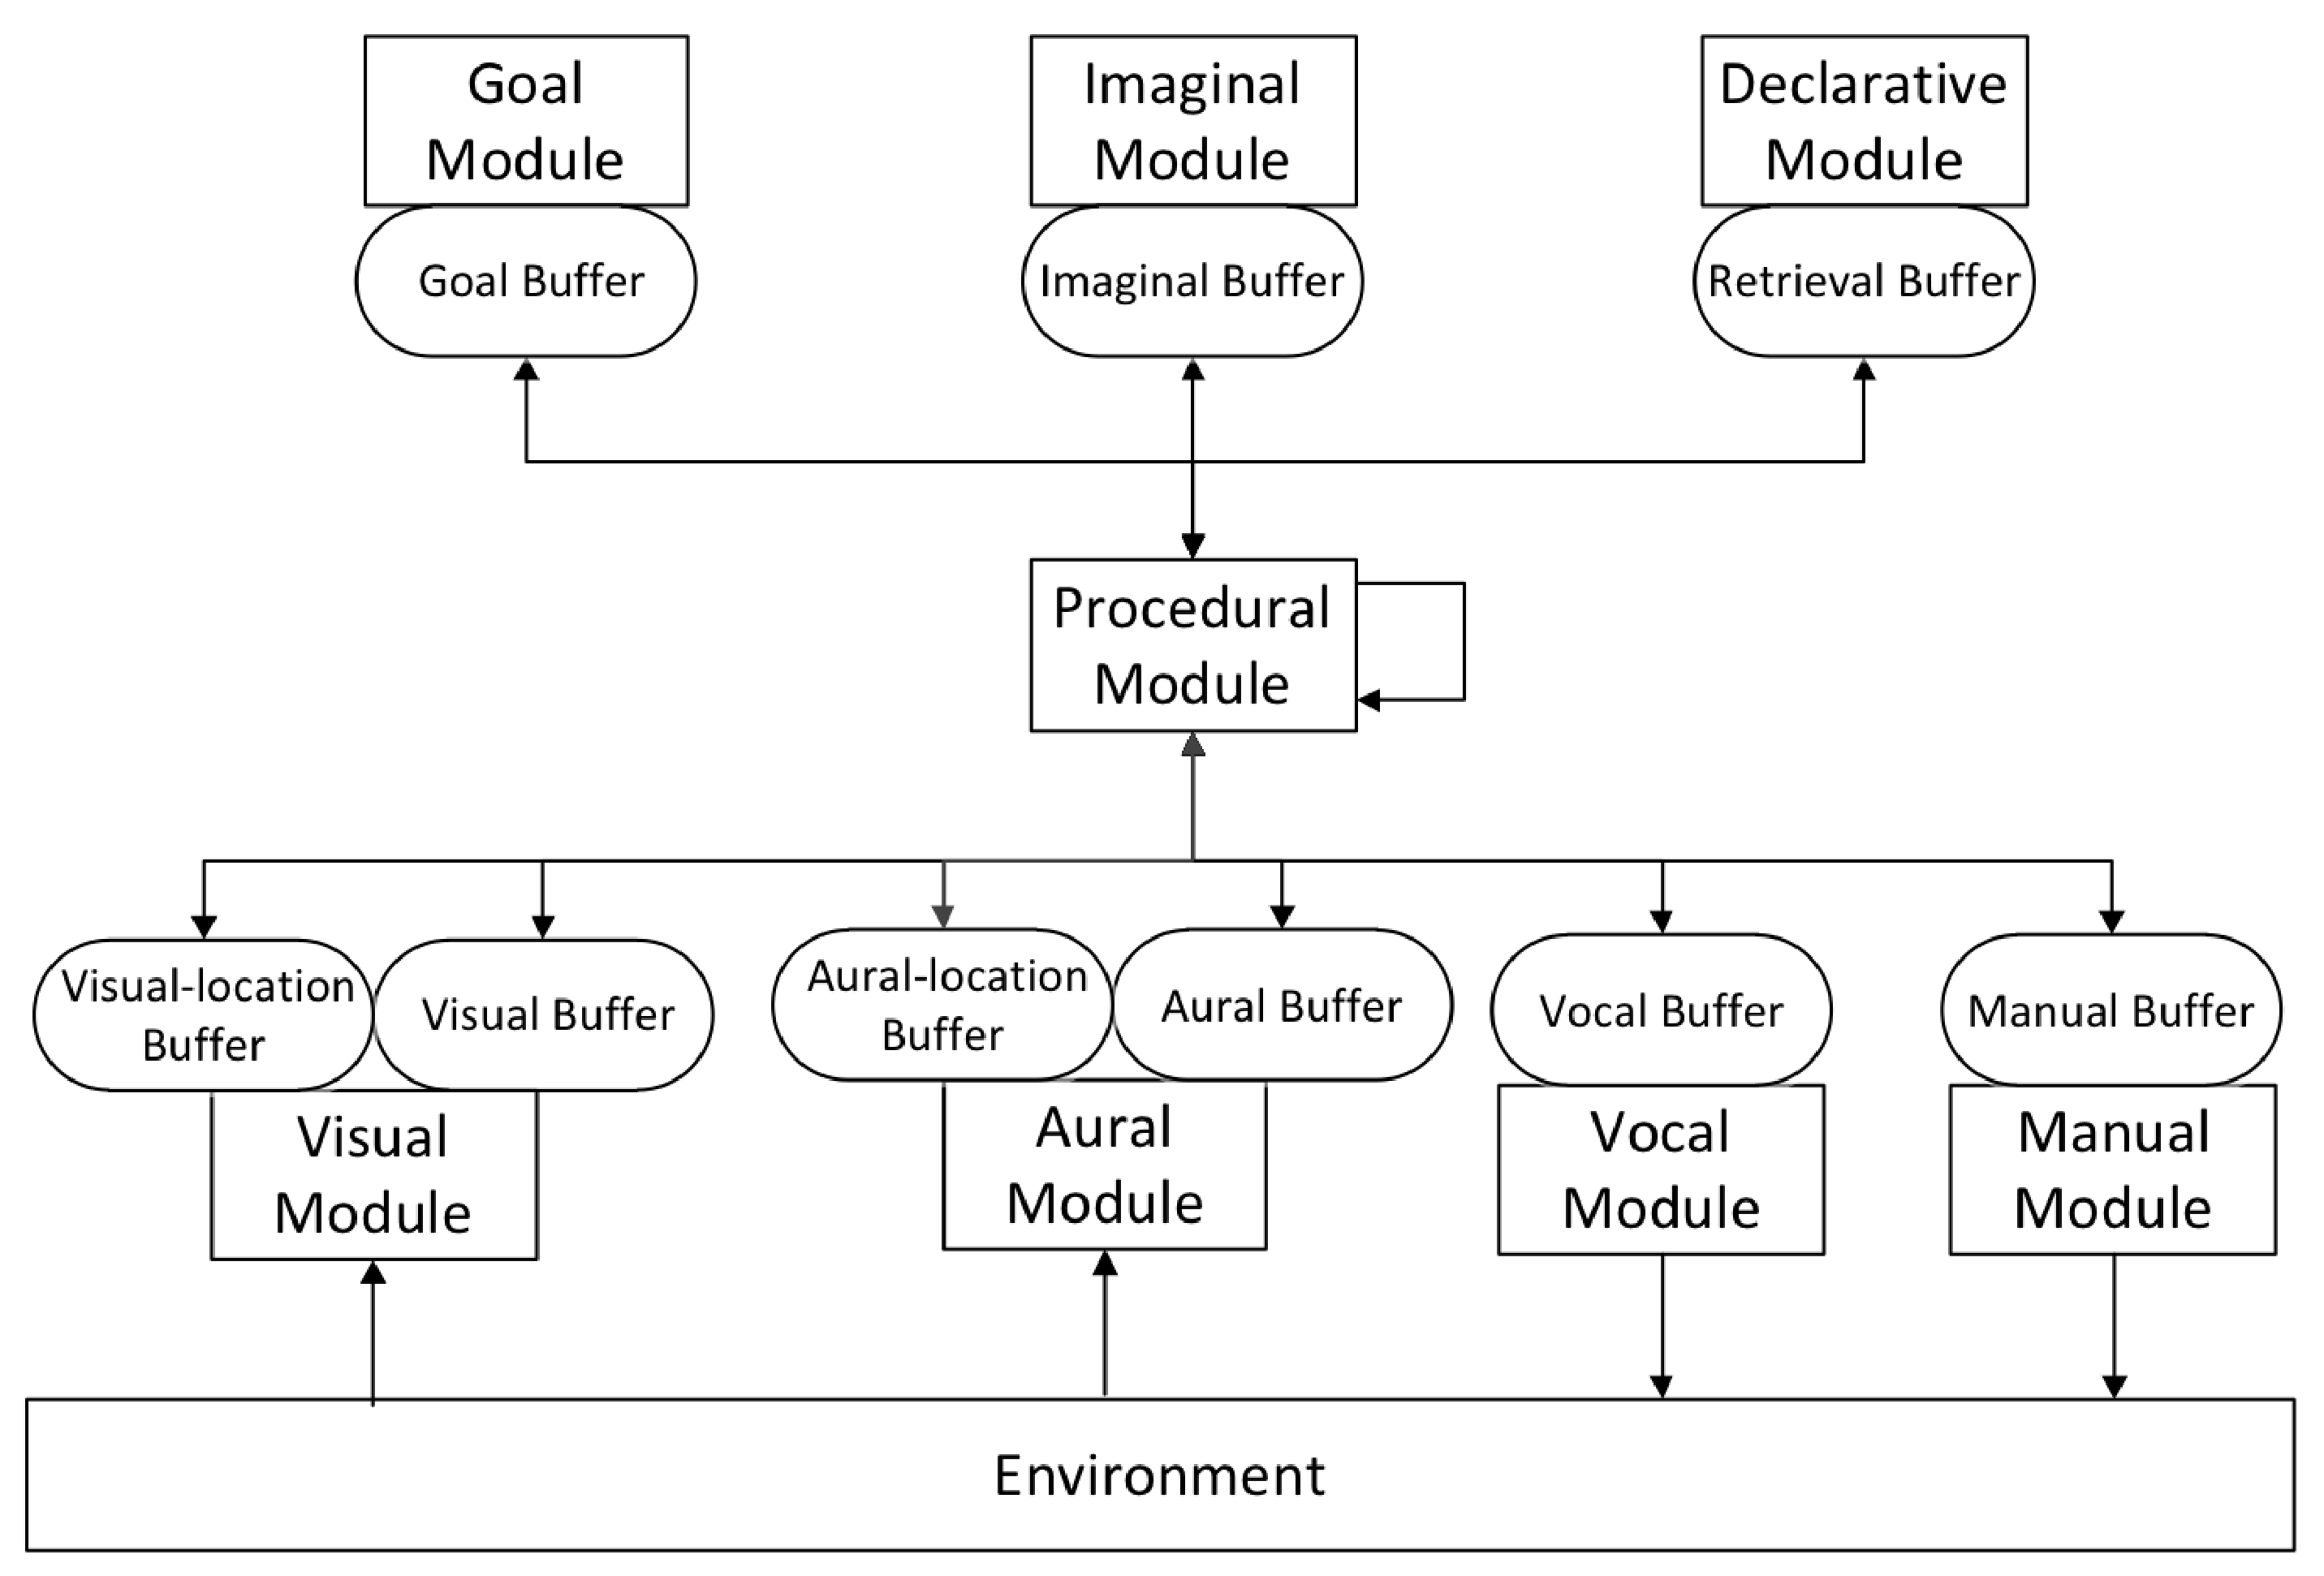
\includegraphics[scale=0.25]{images/ch_01/actr.eps}
	  \end{center} 
	  \caption{\textit{Structure of Act-r.}}  
	  \label{fig:modulesActr}
	\end{figure}
	
	Each module is independent from the others. To communicate one to each other they need to pass through the procedural module. As shown in Figure  ~\ref{fig:modulesActr}, a module can have more than one buffer; for example, the aural module has two buffers: the first is the "Aural-location Buffer", whose function is to get the focus about changes happened in the environment; the second is the "Aural Buffer", to get the real information about the environment.

	The buffers are the built in interface between modules, used to exchange chunks between them. Every buffer belongs to a module, while a module can also have no buffers. Each buffer can hold one chunk at a time, which is readable by the other modules, the guidelines say that a buffer can be written only by its owner. 

	The modules usually work in a parallel way, but their interactions, which are limited to a serial exchange of chunks, can be only serial. There are two reasons for this limitation: firstly the structure of the buffers can hold only one chunk; secondly only one production whose preconditions are satisfied can be fired. When the preconditions of more than one production are satisfied, the one to be fired is the one with the higher priority value,  called \emph{utility value}. This is a numeric quantity, it can be associated with each production in advance or it can be learned while the model runs. \todo{mancano le fonti praticamente ovunque}
	
	\subsection*{Applications}
	Up to now, it has been used in many different areas, the most important of which are problem solving, communication and perception. \todo{espandere e aggiungere fonti}.
	For example, it has been shown that \mbox{ACT-R} can successfully predict \emph{Blood Oxygen Level Dependence} of several parts of the brain, through experiments with \emph{Functional Magnetic Resonance Imaging}. \todo{aggiungere fonti}
	
	
  %% OPENCV
  \section{OpenCV}
	\mbox{OpenCV}, an abbreviation that stands for \emph{Open Source Computer Vision}, is a computer vision library that was originally developed by Intel and, later on, by Willow Garage.
	It is a cross-platform library, released under a BSD license, thus it is free and open source. In the beginning it was developed in C and C++ and afterwards it was expanded by the addition of interfaces for Java and Python. \mbox{OpenCV} is designed for computational efficiency and with a strong focus on real-time applications. The version 2.4 has more than 2500 algorithms. The library has been used in many applications as, for example, mine inspection and robotics \cite{OpenCV:MainWebPage}. The following sections contain a brief history of the library and a list of its main features.
		
	\subsection*{History}
	The \mbox{OpenCV} Project started in 1999 as an Intel Reasearch initiative aimed to improve CPU intensive applications as a part of projects including real-time ray tracing and 3D display walls. The early goals of the project were developing optimized code for basic vision infrastructure, spreading this infrastructure to developers and making it portable and available for free, using a license that let the developers create both commercial and free applications.\newline
	The first alpha version was released to the public in 2000, followed by five beta versions between 2001 and 2005, which lead to version 1.0 in 2006. In 2008, the technology incubator Willow Garage begun supporting the project and, in the same year, version 1.1  was released.
	In October 2009, \mbox{OpenCV} 2.0 was released. It includes many improvements, such as a better C++ interface, more programming patterns, new functions and an optimization for multi-core architectures. According to the current \mbox{OpenCV} release plan, a new version of the library is delivered on a six-months basis. \cite{OpenCV:ChangeLogs}.
	
	\subsection*{Main Features}
	\mbox{OpenCV} offers a wide range of possibilities. First of all, it provides an easy way to manage image and video data types. It also offers functions to load, copy, edit, convert and store images and a basic graphical user interface that lets the developers handle keyboard and mouse and display images and videos. The library lets manipulate images even with matrix and vector algebra routines. It supports the most common dynamic data structures and offers many different basic image processing functions: filtering, edge and corner detection, color conversion, sampling and interpolation, morphological operations, histograms and image pyramids. Beyond this, it integrates many functions for structural analysis of the image, camera calibration, motion analysis and object recognition. \cite{Agam2006}.

\newpage
\chapter{Requirements}

	\section{Functional Requirements}
		The final objective of this work is to make easier the creation of an ACT-R test.\newline
		At the moment, a psychologist, in order to create a test, has to create two interfaces, one for the user and one for ACT-R. The user interface is quite simple, it is formed by simple shapes that can have different colours and words. The user has to read or watch the screen and then choose between a series of possibilities. In order to be analysed by ACT-R, this interface must have a corresponding one, which is simpler and contains only the most important features of the first one. This "simpler" interface is given as input to ACT-R and is written according to a fixed pattern. The figure below shows an example of the user interface of a test and of its corresponding one.\newline \newline	

			%qui metterei le due figure


		The purpose of this work is to create a module which is able to receive as input the user interface, recognize the main features in it and create the corresponding ACT-R interface, which must contain only such features. In order to do this, the software must be made by two parts. The first part will analyze the image. It will recognize and distinguish simple shapes, such as squares, rectangles, circles, stars, arrows; distinguish the colours of the objects; determine the position of each object in the image and recognize the text in the image. The second part will create the correspondent interface for ACT-R, thus... \newline \newline	 %% come deve fare a creare lquestai nterfaccia (lisp o qualcos altro)???? 
		  
		The software is going to be tested with several ACT-R test.
	
	\section{Non Functional Requirements}
	

\newpage
\chapter{Development Process}

	\section{SCRUM}

	\section{Working Instruments}
	In addition to ACT-R and OpenCV, many other tools have been used. Here follows a list of the most important ones.
		\begin{itemize}
		\item \textbf{Eclipse IDE for C/C++ Developers} as \textit{integrated development environment} \footnote{More informations at \url{www.eclipse.org}};
		\item \textbf{Cute} as \textit{unit testing framework} \footnote{More informations at \url{http://cute-test.com}};
		\item \textbf{Mylyn} as \textit{task and application lifecycle management} \footnote{More informations at \url{www.eclipse.org/mylyn}};
		\item \textbf{Trac} as \textit{bug tracking system} \footnote{More informations at \url{trac.edgewall.org}};
		\item \textbf{Git} as \textit{version control system} \footnote{More informations at \url{git-scm.com}}; 
		\item \textbf{Dia} and \textbf{cpp2dia} to create UML diagrams \footnote{More informations at \url{dia-installer.de} and at \url{cpp2dia.sourceforge.net}};
		\item \textbf{ZBar} to read QR codes \footnote{More informations at \url{zbar.sourceforge.net}}.
		%%It can be useful for drawing a large variety of diagrams, in particular UML diagrams, network maps and flowcharts. 
		\end{itemize}

\newpage
\chapter{Project}


\newpage
\chapter{Implementation}




\pagenumbering{roman}


\newpage
\clearpage
\appendix
%\input{Chapters/appendice}
\newpage
\clearpage



%******************************************************************
% Materiale Finale
%******************************************************************
%******************************************************************
%References (two methods in Latex, this (bibTex) with the databe is the best
%******************************************************************
\cleardoublepage
\phantomsection						%gives hyperref something to hold on to when making the link.
\addcontentsline{toc}{chapter}{References}
\bibliographystyle{alpha}				%scelgo come formattare la biblio (abbrv abbrevia i nomi propri. plain non li abbrevia. Ce ne sono un sacco).
\bibliography{beginningEnding/database_references} 	%database dove prendere le info  
\nocite{*}						%stampa TUTTO quello presente nella banca dati, altrimenti solo la roba citata nella tesi

%NB in kile bisogna aggiungere BibTex al QuickBuild per far compilare la bibliografia. Metterlo subito dopo Latex.

\newpage										
\clearpage


\end{document}
